% Created by tikzDevice version 0.12.3.1 on 2022-12-09 11:18:17
% !TEX encoding = UTF-8 Unicode
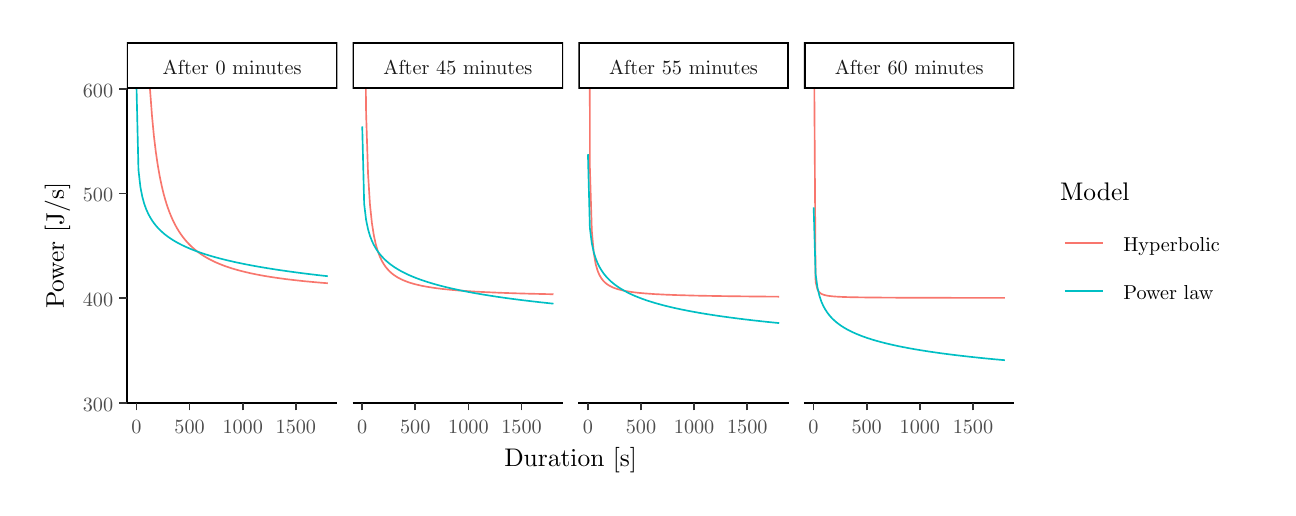
\begin{tikzpicture}[x=1pt,y=1pt]
\definecolor{fillColor}{RGB}{255,255,255}
\path[use as bounding box,fill=fillColor,fill opacity=0.00] (0,0) rectangle (448.07,166.22);
\begin{scope}
\path[clip] (  0.00,  0.00) rectangle (448.07,166.22);
\definecolor{drawColor}{RGB}{255,255,255}
\definecolor{fillColor}{RGB}{255,255,255}

\path[draw=drawColor,line width= 0.6pt,line join=round,line cap=round,fill=fillColor] (  0.00,  0.00) rectangle (448.07,166.22);
\end{scope}
\begin{scope}
\path[clip] ( 35.84, 30.69) rectangle (111.90,144.15);
\definecolor{fillColor}{RGB}{255,255,255}

\path[fill=fillColor] ( 35.84, 30.69) rectangle (111.90,144.15);
\definecolor{drawColor}{RGB}{248,118,109}

\path[draw=drawColor,line width= 0.6pt,line join=round] ( 39.92,1958.52) --
	( 40.03,571.56) --
	( 40.73,326.77) --
	( 41.43,242.23) --
	( 42.12,199.39) --
	( 42.82,173.50) --
	( 43.52,156.16) --
	( 44.22,143.74) --
	( 44.92,134.40) --
	( 45.61,127.12) --
	( 46.31,121.29) --
	( 47.01,116.52) --
	( 47.71,112.53) --
	( 48.41,109.16) --
	( 49.10,106.27) --
	( 49.80,103.76) --
	( 50.50,101.56) --
	( 51.20, 99.63) --
	( 51.90, 97.90) --
	( 52.59, 96.36) --
	( 53.29, 94.97) --
	( 53.99, 93.71) --
	( 54.69, 92.57) --
	( 55.39, 91.53) --
	( 56.08, 90.57) --
	( 56.78, 89.69) --
	( 57.48, 88.88) --
	( 58.18, 88.12) --
	( 58.88, 87.42) --
	( 59.58, 86.77) --
	( 60.27, 86.17) --
	( 60.97, 85.60) --
	( 61.67, 85.06) --
	( 62.37, 84.56) --
	( 63.07, 84.09) --
	( 63.76, 83.65) --
	( 64.46, 83.23) --
	( 65.16, 82.83) --
	( 65.86, 82.45) --
	( 66.56, 82.10) --
	( 67.25, 81.76) --
	( 67.95, 81.43) --
	( 68.65, 81.13) --
	( 69.35, 80.83) --
	( 70.05, 80.55) --
	( 70.74, 80.29) --
	( 71.44, 80.03) --
	( 72.14, 79.79) --
	( 72.84, 79.55) --
	( 73.54, 79.33) --
	( 74.23, 79.11) --
	( 74.93, 78.90) --
	( 75.63, 78.70) --
	( 76.33, 78.51) --
	( 77.03, 78.33) --
	( 77.72, 78.15) --
	( 78.42, 77.98) --
	( 79.12, 77.81) --
	( 79.82, 77.65) --
	( 80.52, 77.49) --
	( 81.21, 77.34) --
	( 81.91, 77.20) --
	( 82.61, 77.06) --
	( 83.31, 76.92) --
	( 84.01, 76.79) --
	( 84.70, 76.67) --
	( 85.40, 76.54) --
	( 86.10, 76.42) --
	( 86.80, 76.31) --
	( 87.50, 76.19) --
	( 88.20, 76.08) --
	( 88.89, 75.98) --
	( 89.59, 75.87) --
	( 90.29, 75.77) --
	( 90.99, 75.67) --
	( 91.69, 75.58) --
	( 92.38, 75.49) --
	( 93.08, 75.39) --
	( 93.78, 75.31) --
	( 94.48, 75.22) --
	( 95.18, 75.14) --
	( 95.87, 75.06) --
	( 96.57, 74.98) --
	( 97.27, 74.90) --
	( 97.97, 74.82) --
	( 98.67, 74.75) --
	( 99.36, 74.67) --
	(100.06, 74.60) --
	(100.76, 74.53) --
	(101.46, 74.47) --
	(102.16, 74.40) --
	(102.85, 74.34) --
	(103.55, 74.27) --
	(104.25, 74.21) --
	(104.95, 74.15) --
	(105.65, 74.09) --
	(106.34, 74.03) --
	(107.04, 73.98) --
	(107.74, 73.92) --
	(108.44, 73.87);
\definecolor{drawColor}{RGB}{0,191,196}

\path[draw=drawColor,line width= 0.6pt,line join=round] ( 39.33,144.69) --
	( 40.03,114.85) --
	( 40.73,108.67) --
	( 41.43,105.09) --
	( 42.12,102.58) --
	( 42.82,100.64) --
	( 43.52, 99.07) --
	( 44.22, 97.75) --
	( 44.92, 96.62) --
	( 45.61, 95.62) --
	( 46.31, 94.73) --
	( 47.01, 93.93) --
	( 47.71, 93.20) --
	( 48.41, 92.54) --
	( 49.10, 91.92) --
	( 49.80, 91.35) --
	( 50.50, 90.82) --
	( 51.20, 90.32) --
	( 51.90, 89.85) --
	( 52.59, 89.41) --
	( 53.29, 88.99) --
	( 53.99, 88.59) --
	( 54.69, 88.21) --
	( 55.39, 87.85) --
	( 56.08, 87.51) --
	( 56.78, 87.18) --
	( 57.48, 86.86) --
	( 58.18, 86.56) --
	( 58.88, 86.27) --
	( 59.58, 85.98) --
	( 60.27, 85.71) --
	( 60.97, 85.45) --
	( 61.67, 85.20) --
	( 62.37, 84.95) --
	( 63.07, 84.71) --
	( 63.76, 84.48) --
	( 64.46, 84.26) --
	( 65.16, 84.04) --
	( 65.86, 83.83) --
	( 66.56, 83.62) --
	( 67.25, 83.42) --
	( 67.95, 83.23) --
	( 68.65, 83.04) --
	( 69.35, 82.85) --
	( 70.05, 82.67) --
	( 70.74, 82.50) --
	( 71.44, 82.32) --
	( 72.14, 82.15) --
	( 72.84, 81.99) --
	( 73.54, 81.83) --
	( 74.23, 81.67) --
	( 74.93, 81.51) --
	( 75.63, 81.36) --
	( 76.33, 81.21) --
	( 77.03, 81.07) --
	( 77.72, 80.93) --
	( 78.42, 80.78) --
	( 79.12, 80.65) --
	( 79.82, 80.51) --
	( 80.52, 80.38) --
	( 81.21, 80.25) --
	( 81.91, 80.12) --
	( 82.61, 79.99) --
	( 83.31, 79.87) --
	( 84.01, 79.75) --
	( 84.70, 79.63) --
	( 85.40, 79.51) --
	( 86.10, 79.40) --
	( 86.80, 79.28) --
	( 87.50, 79.17) --
	( 88.20, 79.06) --
	( 88.89, 78.95) --
	( 89.59, 78.84) --
	( 90.29, 78.73) --
	( 90.99, 78.63) --
	( 91.69, 78.53) --
	( 92.38, 78.43) --
	( 93.08, 78.33) --
	( 93.78, 78.23) --
	( 94.48, 78.13) --
	( 95.18, 78.03) --
	( 95.87, 77.94) --
	( 96.57, 77.84) --
	( 97.27, 77.75) --
	( 97.97, 77.66) --
	( 98.67, 77.57) --
	( 99.36, 77.48) --
	(100.06, 77.39) --
	(100.76, 77.30) --
	(101.46, 77.22) --
	(102.16, 77.13) --
	(102.85, 77.05) --
	(103.55, 76.97) --
	(104.25, 76.88) --
	(104.95, 76.80) --
	(105.65, 76.72) --
	(106.34, 76.64) --
	(107.04, 76.56) --
	(107.74, 76.49) --
	(108.44, 76.41);
\end{scope}
\begin{scope}
\path[clip] (117.40, 30.69) rectangle (193.46,144.15);
\definecolor{fillColor}{RGB}{255,255,255}

\path[fill=fillColor] (117.40, 30.69) rectangle (193.46,144.15);
\definecolor{drawColor}{RGB}{248,118,109}

\path[draw=drawColor,line width= 0.6pt,line join=round] (121.07,1958.52) --
	(121.59,198.71) --
	(122.29,135.35) --
	(122.99,113.47) --
	(123.68,102.38) --
	(124.38, 95.68) --
	(125.08, 91.19) --
	(125.78, 87.98) --
	(126.48, 85.56) --
	(127.17, 83.68) --
	(127.87, 82.17) --
	(128.57, 80.93) --
	(129.27, 79.90) --
	(129.97, 79.03) --
	(130.66, 78.28) --
	(131.36, 77.63) --
	(132.06, 77.06) --
	(132.76, 76.56) --
	(133.46, 76.12) --
	(134.15, 75.72) --
	(134.85, 75.36) --
	(135.55, 75.03) --
	(136.25, 74.74) --
	(136.95, 74.47) --
	(137.64, 74.22) --
	(138.34, 73.99) --
	(139.04, 73.78) --
	(139.74, 73.58) --
	(140.44, 73.40) --
	(141.13, 73.24) --
	(141.83, 73.08) --
	(142.53, 72.93) --
	(143.23, 72.79) --
	(143.93, 72.66) --
	(144.63, 72.54) --
	(145.32, 72.43) --
	(146.02, 72.32) --
	(146.72, 72.21) --
	(147.42, 72.12) --
	(148.12, 72.02) --
	(148.81, 71.94) --
	(149.51, 71.85) --
	(150.21, 71.77) --
	(150.91, 71.70) --
	(151.61, 71.63) --
	(152.30, 71.56) --
	(153.00, 71.49) --
	(153.70, 71.43) --
	(154.40, 71.37) --
	(155.10, 71.31) --
	(155.79, 71.25) --
	(156.49, 71.20) --
	(157.19, 71.15) --
	(157.89, 71.10) --
	(158.59, 71.05) --
	(159.28, 71.00) --
	(159.98, 70.96) --
	(160.68, 70.91) --
	(161.38, 70.87) --
	(162.08, 70.83) --
	(162.77, 70.79) --
	(163.47, 70.76) --
	(164.17, 70.72) --
	(164.87, 70.69) --
	(165.57, 70.65) --
	(166.26, 70.62) --
	(166.96, 70.59) --
	(167.66, 70.56) --
	(168.36, 70.53) --
	(169.06, 70.50) --
	(169.75, 70.47) --
	(170.45, 70.44) --
	(171.15, 70.41) --
	(171.85, 70.39) --
	(172.55, 70.36) --
	(173.25, 70.34) --
	(173.94, 70.31) --
	(174.64, 70.29) --
	(175.34, 70.27) --
	(176.04, 70.24) --
	(176.74, 70.22) --
	(177.43, 70.20) --
	(178.13, 70.18) --
	(178.83, 70.16) --
	(179.53, 70.14) --
	(180.23, 70.12) --
	(180.92, 70.10) --
	(181.62, 70.09) --
	(182.32, 70.07) --
	(183.02, 70.05) --
	(183.72, 70.03) --
	(184.41, 70.02) --
	(185.11, 70.00) --
	(185.81, 69.98) --
	(186.51, 69.97) --
	(187.21, 69.95) --
	(187.90, 69.94) --
	(188.60, 69.92) --
	(189.30, 69.91) --
	(190.00, 69.89);
\definecolor{drawColor}{RGB}{0,191,196}

\path[draw=drawColor,line width= 0.6pt,line join=round] (120.89,130.51) --
	(121.59,102.53) --
	(122.29, 96.74) --
	(122.99, 93.38) --
	(123.68, 91.02) --
	(124.38, 89.21) --
	(125.08, 87.73) --
	(125.78, 86.50) --
	(126.48, 85.43) --
	(127.17, 84.50) --
	(127.87, 83.67) --
	(128.57, 82.92) --
	(129.27, 82.23) --
	(129.97, 81.61) --
	(130.66, 81.03) --
	(131.36, 80.50) --
	(132.06, 80.00) --
	(132.76, 79.53) --
	(133.46, 79.09) --
	(134.15, 78.68) --
	(134.85, 78.28) --
	(135.55, 77.91) --
	(136.25, 77.56) --
	(136.95, 77.22) --
	(137.64, 76.89) --
	(138.34, 76.58) --
	(139.04, 76.29) --
	(139.74, 76.00) --
	(140.44, 75.73) --
	(141.13, 75.46) --
	(141.83, 75.21) --
	(142.53, 74.96) --
	(143.23, 74.73) --
	(143.93, 74.50) --
	(144.63, 74.27) --
	(145.32, 74.06) --
	(146.02, 73.85) --
	(146.72, 73.64) --
	(147.42, 73.44) --
	(148.12, 73.25) --
	(148.81, 73.06) --
	(149.51, 72.88) --
	(150.21, 72.70) --
	(150.91, 72.53) --
	(151.61, 72.36) --
	(152.30, 72.19) --
	(153.00, 72.03) --
	(153.70, 71.87) --
	(154.40, 71.72) --
	(155.10, 71.57) --
	(155.79, 71.42) --
	(156.49, 71.27) --
	(157.19, 71.13) --
	(157.89, 70.99) --
	(158.59, 70.85) --
	(159.28, 70.72) --
	(159.98, 70.59) --
	(160.68, 70.46) --
	(161.38, 70.33) --
	(162.08, 70.21) --
	(162.77, 70.09) --
	(163.47, 69.97) --
	(164.17, 69.85) --
	(164.87, 69.73) --
	(165.57, 69.62) --
	(166.26, 69.51) --
	(166.96, 69.39) --
	(167.66, 69.29) --
	(168.36, 69.18) --
	(169.06, 69.07) --
	(169.75, 68.97) --
	(170.45, 68.87) --
	(171.15, 68.77) --
	(171.85, 68.67) --
	(172.55, 68.57) --
	(173.25, 68.47) --
	(173.94, 68.38) --
	(174.64, 68.28) --
	(175.34, 68.19) --
	(176.04, 68.10) --
	(176.74, 68.01) --
	(177.43, 67.92) --
	(178.13, 67.83) --
	(178.83, 67.74) --
	(179.53, 67.66) --
	(180.23, 67.57) --
	(180.92, 67.49) --
	(181.62, 67.41) --
	(182.32, 67.33) --
	(183.02, 67.25) --
	(183.72, 67.17) --
	(184.41, 67.09) --
	(185.11, 67.01) --
	(185.81, 66.93) --
	(186.51, 66.86) --
	(187.21, 66.78) --
	(187.90, 66.71) --
	(188.60, 66.63) --
	(189.30, 66.56) --
	(190.00, 66.49);
\end{scope}
\begin{scope}
\path[clip] (198.96, 30.69) rectangle (275.02,144.15);
\definecolor{fillColor}{RGB}{255,255,255}

\path[fill=fillColor] (198.96, 30.69) rectangle (275.02,144.15);
\definecolor{drawColor}{RGB}{248,118,109}

\path[draw=drawColor,line width= 0.6pt,line join=round] (202.45,976.22) --
	(203.15,115.85) --
	(203.85, 92.81) --
	(204.55, 84.86) --
	(205.24, 80.83) --
	(205.94, 78.39) --
	(206.64, 76.76) --
	(207.34, 75.59) --
	(208.04, 74.71) --
	(208.73, 74.02) --
	(209.43, 73.48) --
	(210.13, 73.03) --
	(210.83, 72.65) --
	(211.53, 72.33) --
	(212.22, 72.06) --
	(212.92, 71.83) --
	(213.62, 71.62) --
	(214.32, 71.44) --
	(215.02, 71.27) --
	(215.71, 71.13) --
	(216.41, 71.00) --
	(217.11, 70.88) --
	(217.81, 70.77) --
	(218.51, 70.67) --
	(219.20, 70.58) --
	(219.90, 70.50) --
	(220.60, 70.42) --
	(221.30, 70.35) --
	(222.00, 70.29) --
	(222.69, 70.23) --
	(223.39, 70.17) --
	(224.09, 70.12) --
	(224.79, 70.07) --
	(225.49, 70.02) --
	(226.19, 69.97) --
	(226.88, 69.93) --
	(227.58, 69.89) --
	(228.28, 69.86) --
	(228.98, 69.82) --
	(229.68, 69.79) --
	(230.37, 69.75) --
	(231.07, 69.72) --
	(231.77, 69.69) --
	(232.47, 69.67) --
	(233.17, 69.64) --
	(233.86, 69.62) --
	(234.56, 69.59) --
	(235.26, 69.57) --
	(235.96, 69.55) --
	(236.66, 69.53) --
	(237.35, 69.51) --
	(238.05, 69.49) --
	(238.75, 69.47) --
	(239.45, 69.45) --
	(240.15, 69.43) --
	(240.84, 69.41) --
	(241.54, 69.40) --
	(242.24, 69.38) --
	(242.94, 69.37) --
	(243.64, 69.35) --
	(244.33, 69.34) --
	(245.03, 69.33) --
	(245.73, 69.31) --
	(246.43, 69.30) --
	(247.13, 69.29) --
	(247.82, 69.27) --
	(248.52, 69.26) --
	(249.22, 69.25) --
	(249.92, 69.24) --
	(250.62, 69.23) --
	(251.31, 69.22) --
	(252.01, 69.21) --
	(252.71, 69.20) --
	(253.41, 69.19) --
	(254.11, 69.18) --
	(254.81, 69.17) --
	(255.50, 69.16) --
	(256.20, 69.16) --
	(256.90, 69.15) --
	(257.60, 69.14) --
	(258.30, 69.13) --
	(258.99, 69.12) --
	(259.69, 69.12) --
	(260.39, 69.11) --
	(261.09, 69.10) --
	(261.79, 69.09) --
	(262.48, 69.09) --
	(263.18, 69.08) --
	(263.88, 69.07) --
	(264.58, 69.07) --
	(265.28, 69.06) --
	(265.97, 69.06) --
	(266.67, 69.05) --
	(267.37, 69.04) --
	(268.07, 69.04) --
	(268.77, 69.03) --
	(269.46, 69.03) --
	(270.16, 69.02) --
	(270.86, 69.02) --
	(271.56, 69.01);
\definecolor{drawColor}{RGB}{0,191,196}

\path[draw=drawColor,line width= 0.6pt,line join=round] (202.45,120.48) --
	(203.15, 93.81) --
	(203.85, 88.30) --
	(204.55, 85.10) --
	(205.24, 82.85) --
	(205.94, 81.12) --
	(206.64, 79.72) --
	(207.34, 78.54) --
	(208.04, 77.52) --
	(208.73, 76.63) --
	(209.43, 75.84) --
	(210.13, 75.12) --
	(210.83, 74.47) --
	(211.53, 73.88) --
	(212.22, 73.33) --
	(212.92, 72.82) --
	(213.62, 72.34) --
	(214.32, 71.90) --
	(215.02, 71.48) --
	(215.71, 71.08) --
	(216.41, 70.71) --
	(217.11, 70.35) --
	(217.81, 70.01) --
	(218.51, 69.69) --
	(219.20, 69.38) --
	(219.90, 69.09) --
	(220.60, 68.81) --
	(221.30, 68.54) --
	(222.00, 68.27) --
	(222.69, 68.02) --
	(223.39, 67.78) --
	(224.09, 67.54) --
	(224.79, 67.32) --
	(225.49, 67.10) --
	(226.19, 66.89) --
	(226.88, 66.68) --
	(227.58, 66.48) --
	(228.28, 66.29) --
	(228.98, 66.10) --
	(229.68, 65.91) --
	(230.37, 65.73) --
	(231.07, 65.56) --
	(231.77, 65.39) --
	(232.47, 65.22) --
	(233.17, 65.06) --
	(233.86, 64.90) --
	(234.56, 64.75) --
	(235.26, 64.60) --
	(235.96, 64.45) --
	(236.66, 64.31) --
	(237.35, 64.17) --
	(238.05, 64.03) --
	(238.75, 63.89) --
	(239.45, 63.76) --
	(240.15, 63.63) --
	(240.84, 63.50) --
	(241.54, 63.38) --
	(242.24, 63.25) --
	(242.94, 63.13) --
	(243.64, 63.01) --
	(244.33, 62.90) --
	(245.03, 62.78) --
	(245.73, 62.67) --
	(246.43, 62.56) --
	(247.13, 62.45) --
	(247.82, 62.34) --
	(248.52, 62.24) --
	(249.22, 62.13) --
	(249.92, 62.03) --
	(250.62, 61.93) --
	(251.31, 61.83) --
	(252.01, 61.74) --
	(252.71, 61.64) --
	(253.41, 61.54) --
	(254.11, 61.45) --
	(254.81, 61.36) --
	(255.50, 61.27) --
	(256.20, 61.18) --
	(256.90, 61.09) --
	(257.60, 61.00) --
	(258.30, 60.92) --
	(258.99, 60.83) --
	(259.69, 60.75) --
	(260.39, 60.67) --
	(261.09, 60.58) --
	(261.79, 60.50) --
	(262.48, 60.42) --
	(263.18, 60.34) --
	(263.88, 60.27) --
	(264.58, 60.19) --
	(265.28, 60.11) --
	(265.97, 60.04) --
	(266.67, 59.96) --
	(267.37, 59.89) --
	(268.07, 59.82) --
	(268.77, 59.75) --
	(269.46, 59.68) --
	(270.16, 59.61) --
	(270.86, 59.54) --
	(271.56, 59.47);
\end{scope}
\begin{scope}
\path[clip] (280.52, 30.69) rectangle (356.58,144.15);
\definecolor{fillColor}{RGB}{255,255,255}

\path[fill=fillColor] (280.52, 30.69) rectangle (356.58,144.15);
\definecolor{drawColor}{RGB}{248,118,109}

\path[draw=drawColor,line width= 0.6pt,line join=round] (284.01,181.97) --
	(284.71, 74.43) --
	(285.41, 71.55) --
	(286.11, 70.55) --
	(286.80, 70.05) --
	(287.50, 69.74) --
	(288.20, 69.54) --
	(288.90, 69.39) --
	(289.60, 69.28) --
	(290.29, 69.20) --
	(290.99, 69.13) --
	(291.69, 69.07) --
	(292.39, 69.03) --
	(293.09, 68.99) --
	(293.78, 68.95) --
	(294.48, 68.92) --
	(295.18, 68.90) --
	(295.88, 68.87) --
	(296.58, 68.85) --
	(297.27, 68.83) --
	(297.97, 68.82) --
	(298.67, 68.80) --
	(299.37, 68.79) --
	(300.07, 68.78) --
	(300.76, 68.77) --
	(301.46, 68.76) --
	(302.16, 68.75) --
	(302.86, 68.74) --
	(303.56, 68.73) --
	(304.25, 68.72) --
	(304.95, 68.71) --
	(305.65, 68.71) --
	(306.35, 68.70) --
	(307.05, 68.70) --
	(307.74, 68.69) --
	(308.44, 68.69) --
	(309.14, 68.68) --
	(309.84, 68.68) --
	(310.54, 68.67) --
	(311.24, 68.67) --
	(311.93, 68.66) --
	(312.63, 68.66) --
	(313.33, 68.66) --
	(314.03, 68.65) --
	(314.73, 68.65) --
	(315.42, 68.65) --
	(316.12, 68.64) --
	(316.82, 68.64) --
	(317.52, 68.64) --
	(318.22, 68.63) --
	(318.91, 68.63) --
	(319.61, 68.63) --
	(320.31, 68.63) --
	(321.01, 68.62) --
	(321.71, 68.62) --
	(322.40, 68.62) --
	(323.10, 68.62) --
	(323.80, 68.62) --
	(324.50, 68.61) --
	(325.20, 68.61) --
	(325.89, 68.61) --
	(326.59, 68.61) --
	(327.29, 68.61) --
	(327.99, 68.61) --
	(328.69, 68.60) --
	(329.38, 68.60) --
	(330.08, 68.60) --
	(330.78, 68.60) --
	(331.48, 68.60) --
	(332.18, 68.60) --
	(332.87, 68.60) --
	(333.57, 68.60) --
	(334.27, 68.59) --
	(334.97, 68.59) --
	(335.67, 68.59) --
	(336.36, 68.59) --
	(337.06, 68.59) --
	(337.76, 68.59) --
	(338.46, 68.59) --
	(339.16, 68.59) --
	(339.86, 68.59) --
	(340.55, 68.58) --
	(341.25, 68.58) --
	(341.95, 68.58) --
	(342.65, 68.58) --
	(343.35, 68.58) --
	(344.04, 68.58) --
	(344.74, 68.58) --
	(345.44, 68.58) --
	(346.14, 68.58) --
	(346.84, 68.58) --
	(347.53, 68.58) --
	(348.23, 68.57) --
	(348.93, 68.57) --
	(349.63, 68.57) --
	(350.33, 68.57) --
	(351.02, 68.57) --
	(351.72, 68.57) --
	(352.42, 68.57) --
	(353.12, 68.57);
\definecolor{drawColor}{RGB}{0,191,196}

\path[draw=drawColor,line width= 0.6pt,line join=round] (284.01,101.32) --
	(284.71, 77.17) --
	(285.41, 72.17) --
	(286.11, 69.27) --
	(286.80, 67.23) --
	(287.50, 65.67) --
	(288.20, 64.40) --
	(288.90, 63.33) --
	(289.60, 62.41) --
	(290.29, 61.60) --
	(290.99, 60.88) --
	(291.69, 60.24) --
	(292.39, 59.65) --
	(293.09, 59.11) --
	(293.78, 58.61) --
	(294.48, 58.15) --
	(295.18, 57.72) --
	(295.88, 57.31) --
	(296.58, 56.93) --
	(297.27, 56.58) --
	(297.97, 56.24) --
	(298.67, 55.92) --
	(299.37, 55.61) --
	(300.07, 55.32) --
	(300.76, 55.04) --
	(301.46, 54.77) --
	(302.16, 54.52) --
	(302.86, 54.27) --
	(303.56, 54.03) --
	(304.25, 53.81) --
	(304.95, 53.59) --
	(305.65, 53.37) --
	(306.35, 53.17) --
	(307.05, 52.97) --
	(307.74, 52.78) --
	(308.44, 52.59) --
	(309.14, 52.41) --
	(309.84, 52.23) --
	(310.54, 52.06) --
	(311.24, 51.90) --
	(311.93, 51.73) --
	(312.63, 51.58) --
	(313.33, 51.42) --
	(314.03, 51.27) --
	(314.73, 51.12) --
	(315.42, 50.98) --
	(316.12, 50.84) --
	(316.82, 50.71) --
	(317.52, 50.57) --
	(318.22, 50.44) --
	(318.91, 50.31) --
	(319.61, 50.19) --
	(320.31, 50.06) --
	(321.01, 49.94) --
	(321.71, 49.83) --
	(322.40, 49.71) --
	(323.10, 49.60) --
	(323.80, 49.49) --
	(324.50, 49.38) --
	(325.20, 49.27) --
	(325.89, 49.16) --
	(326.59, 49.06) --
	(327.29, 48.96) --
	(327.99, 48.86) --
	(328.69, 48.76) --
	(329.38, 48.66) --
	(330.08, 48.57) --
	(330.78, 48.47) --
	(331.48, 48.38) --
	(332.18, 48.29) --
	(332.87, 48.20) --
	(333.57, 48.11) --
	(334.27, 48.02) --
	(334.97, 47.94) --
	(335.67, 47.85) --
	(336.36, 47.77) --
	(337.06, 47.69) --
	(337.76, 47.61) --
	(338.46, 47.53) --
	(339.16, 47.45) --
	(339.86, 47.37) --
	(340.55, 47.29) --
	(341.25, 47.22) --
	(341.95, 47.14) --
	(342.65, 47.07) --
	(343.35, 46.99) --
	(344.04, 46.92) --
	(344.74, 46.85) --
	(345.44, 46.78) --
	(346.14, 46.71) --
	(346.84, 46.64) --
	(347.53, 46.57) --
	(348.23, 46.51) --
	(348.93, 46.44) --
	(349.63, 46.37) --
	(350.33, 46.31) --
	(351.02, 46.25) --
	(351.72, 46.18) --
	(352.42, 46.12) --
	(353.12, 46.06);
\end{scope}
\begin{scope}
\path[clip] ( 35.84,144.15) rectangle (111.90,160.72);
\definecolor{drawColor}{RGB}{0,0,0}
\definecolor{fillColor}{RGB}{255,255,255}

\path[draw=drawColor,line width= 1.1pt,line join=round,line cap=round,fill=fillColor] ( 35.84,144.15) rectangle (111.90,160.72);
\definecolor{drawColor}{gray}{0.10}

\node[text=drawColor,anchor=base,inner sep=0pt, outer sep=0pt, scale=  0.73] at ( 73.87,149.41) {After 0 minutes};
\end{scope}
\begin{scope}
\path[clip] (117.40,144.15) rectangle (193.46,160.72);
\definecolor{drawColor}{RGB}{0,0,0}
\definecolor{fillColor}{RGB}{255,255,255}

\path[draw=drawColor,line width= 1.1pt,line join=round,line cap=round,fill=fillColor] (117.40,144.15) rectangle (193.46,160.72);
\definecolor{drawColor}{gray}{0.10}

\node[text=drawColor,anchor=base,inner sep=0pt, outer sep=0pt, scale=  0.73] at (155.43,149.41) {After 45 minutes};
\end{scope}
\begin{scope}
\path[clip] (198.96,144.15) rectangle (275.02,160.72);
\definecolor{drawColor}{RGB}{0,0,0}
\definecolor{fillColor}{RGB}{255,255,255}

\path[draw=drawColor,line width= 1.1pt,line join=round,line cap=round,fill=fillColor] (198.96,144.15) rectangle (275.02,160.72);
\definecolor{drawColor}{gray}{0.10}

\node[text=drawColor,anchor=base,inner sep=0pt, outer sep=0pt, scale=  0.73] at (236.99,149.41) {After 55 minutes};
\end{scope}
\begin{scope}
\path[clip] (280.52,144.15) rectangle (356.58,160.72);
\definecolor{drawColor}{RGB}{0,0,0}
\definecolor{fillColor}{RGB}{255,255,255}

\path[draw=drawColor,line width= 1.1pt,line join=round,line cap=round,fill=fillColor] (280.52,144.15) rectangle (356.58,160.72);
\definecolor{drawColor}{gray}{0.10}

\node[text=drawColor,anchor=base,inner sep=0pt, outer sep=0pt, scale=  0.73] at (318.55,149.41) {After 60 minutes};
\end{scope}
\begin{scope}
\path[clip] (  0.00,  0.00) rectangle (448.07,166.22);
\definecolor{drawColor}{RGB}{0,0,0}

\path[draw=drawColor,line width= 0.6pt,line join=round] ( 35.84, 30.69) --
	(111.90, 30.69);
\end{scope}
\begin{scope}
\path[clip] (  0.00,  0.00) rectangle (448.07,166.22);
\definecolor{drawColor}{gray}{0.20}

\path[draw=drawColor,line width= 0.6pt,line join=round] ( 39.29, 27.94) --
	( 39.29, 30.69);

\path[draw=drawColor,line width= 0.6pt,line join=round] ( 58.50, 27.94) --
	( 58.50, 30.69);

\path[draw=drawColor,line width= 0.6pt,line join=round] ( 77.71, 27.94) --
	( 77.71, 30.69);

\path[draw=drawColor,line width= 0.6pt,line join=round] ( 96.91, 27.94) --
	( 96.91, 30.69);
\end{scope}
\begin{scope}
\path[clip] (  0.00,  0.00) rectangle (448.07,166.22);
\definecolor{drawColor}{gray}{0.30}

\node[text=drawColor,anchor=base,inner sep=0pt, outer sep=0pt, scale=  0.73] at ( 39.29, 19.68) {0};

\node[text=drawColor,anchor=base,inner sep=0pt, outer sep=0pt, scale=  0.73] at ( 58.50, 19.68) {500};

\node[text=drawColor,anchor=base,inner sep=0pt, outer sep=0pt, scale=  0.73] at ( 77.71, 19.68) {1000};

\node[text=drawColor,anchor=base,inner sep=0pt, outer sep=0pt, scale=  0.73] at ( 96.91, 19.68) {1500};
\end{scope}
\begin{scope}
\path[clip] (  0.00,  0.00) rectangle (448.07,166.22);
\definecolor{drawColor}{RGB}{0,0,0}

\path[draw=drawColor,line width= 0.6pt,line join=round] (117.40, 30.69) --
	(193.46, 30.69);
\end{scope}
\begin{scope}
\path[clip] (  0.00,  0.00) rectangle (448.07,166.22);
\definecolor{drawColor}{gray}{0.20}

\path[draw=drawColor,line width= 0.6pt,line join=round] (120.85, 27.94) --
	(120.85, 30.69);

\path[draw=drawColor,line width= 0.6pt,line join=round] (140.06, 27.94) --
	(140.06, 30.69);

\path[draw=drawColor,line width= 0.6pt,line join=round] (159.27, 27.94) --
	(159.27, 30.69);

\path[draw=drawColor,line width= 0.6pt,line join=round] (178.47, 27.94) --
	(178.47, 30.69);
\end{scope}
\begin{scope}
\path[clip] (  0.00,  0.00) rectangle (448.07,166.22);
\definecolor{drawColor}{gray}{0.30}

\node[text=drawColor,anchor=base,inner sep=0pt, outer sep=0pt, scale=  0.73] at (120.85, 19.68) {0};

\node[text=drawColor,anchor=base,inner sep=0pt, outer sep=0pt, scale=  0.73] at (140.06, 19.68) {500};

\node[text=drawColor,anchor=base,inner sep=0pt, outer sep=0pt, scale=  0.73] at (159.27, 19.68) {1000};

\node[text=drawColor,anchor=base,inner sep=0pt, outer sep=0pt, scale=  0.73] at (178.47, 19.68) {1500};
\end{scope}
\begin{scope}
\path[clip] (  0.00,  0.00) rectangle (448.07,166.22);
\definecolor{drawColor}{RGB}{0,0,0}

\path[draw=drawColor,line width= 0.6pt,line join=round] (198.96, 30.69) --
	(275.02, 30.69);
\end{scope}
\begin{scope}
\path[clip] (  0.00,  0.00) rectangle (448.07,166.22);
\definecolor{drawColor}{gray}{0.20}

\path[draw=drawColor,line width= 0.6pt,line join=round] (202.41, 27.94) --
	(202.41, 30.69);

\path[draw=drawColor,line width= 0.6pt,line join=round] (221.62, 27.94) --
	(221.62, 30.69);

\path[draw=drawColor,line width= 0.6pt,line join=round] (240.83, 27.94) --
	(240.83, 30.69);

\path[draw=drawColor,line width= 0.6pt,line join=round] (260.03, 27.94) --
	(260.03, 30.69);
\end{scope}
\begin{scope}
\path[clip] (  0.00,  0.00) rectangle (448.07,166.22);
\definecolor{drawColor}{gray}{0.30}

\node[text=drawColor,anchor=base,inner sep=0pt, outer sep=0pt, scale=  0.73] at (202.41, 19.68) {0};

\node[text=drawColor,anchor=base,inner sep=0pt, outer sep=0pt, scale=  0.73] at (221.62, 19.68) {500};

\node[text=drawColor,anchor=base,inner sep=0pt, outer sep=0pt, scale=  0.73] at (240.83, 19.68) {1000};

\node[text=drawColor,anchor=base,inner sep=0pt, outer sep=0pt, scale=  0.73] at (260.03, 19.68) {1500};
\end{scope}
\begin{scope}
\path[clip] (  0.00,  0.00) rectangle (448.07,166.22);
\definecolor{drawColor}{RGB}{0,0,0}

\path[draw=drawColor,line width= 0.6pt,line join=round] (280.52, 30.69) --
	(356.58, 30.69);
\end{scope}
\begin{scope}
\path[clip] (  0.00,  0.00) rectangle (448.07,166.22);
\definecolor{drawColor}{gray}{0.20}

\path[draw=drawColor,line width= 0.6pt,line join=round] (283.97, 27.94) --
	(283.97, 30.69);

\path[draw=drawColor,line width= 0.6pt,line join=round] (303.18, 27.94) --
	(303.18, 30.69);

\path[draw=drawColor,line width= 0.6pt,line join=round] (322.39, 27.94) --
	(322.39, 30.69);

\path[draw=drawColor,line width= 0.6pt,line join=round] (341.59, 27.94) --
	(341.59, 30.69);
\end{scope}
\begin{scope}
\path[clip] (  0.00,  0.00) rectangle (448.07,166.22);
\definecolor{drawColor}{gray}{0.30}

\node[text=drawColor,anchor=base,inner sep=0pt, outer sep=0pt, scale=  0.73] at (283.97, 19.68) {0};

\node[text=drawColor,anchor=base,inner sep=0pt, outer sep=0pt, scale=  0.73] at (303.18, 19.68) {500};

\node[text=drawColor,anchor=base,inner sep=0pt, outer sep=0pt, scale=  0.73] at (322.39, 19.68) {1000};

\node[text=drawColor,anchor=base,inner sep=0pt, outer sep=0pt, scale=  0.73] at (341.59, 19.68) {1500};
\end{scope}
\begin{scope}
\path[clip] (  0.00,  0.00) rectangle (448.07,166.22);
\definecolor{drawColor}{RGB}{0,0,0}

\path[draw=drawColor,line width= 0.6pt,line join=round] ( 35.84, 30.69) --
	( 35.84,144.15);
\end{scope}
\begin{scope}
\path[clip] (  0.00,  0.00) rectangle (448.07,166.22);
\definecolor{drawColor}{gray}{0.30}

\node[text=drawColor,anchor=base east,inner sep=0pt, outer sep=0pt, scale=  0.73] at ( 30.89, 27.66) {300};

\node[text=drawColor,anchor=base east,inner sep=0pt, outer sep=0pt, scale=  0.73] at ( 30.89, 65.48) {400};

\node[text=drawColor,anchor=base east,inner sep=0pt, outer sep=0pt, scale=  0.73] at ( 30.89,103.30) {500};

\node[text=drawColor,anchor=base east,inner sep=0pt, outer sep=0pt, scale=  0.73] at ( 30.89,141.12) {600};
\end{scope}
\begin{scope}
\path[clip] (  0.00,  0.00) rectangle (448.07,166.22);
\definecolor{drawColor}{gray}{0.20}

\path[draw=drawColor,line width= 0.6pt,line join=round] ( 33.09, 30.69) --
	( 35.84, 30.69);

\path[draw=drawColor,line width= 0.6pt,line join=round] ( 33.09, 68.51) --
	( 35.84, 68.51);

\path[draw=drawColor,line width= 0.6pt,line join=round] ( 33.09,106.33) --
	( 35.84,106.33);

\path[draw=drawColor,line width= 0.6pt,line join=round] ( 33.09,144.15) --
	( 35.84,144.15);
\end{scope}
\begin{scope}
\path[clip] (  0.00,  0.00) rectangle (448.07,166.22);
\definecolor{drawColor}{RGB}{0,0,0}

\node[text=drawColor,anchor=base,inner sep=0pt, outer sep=0pt, scale=  0.92] at (196.21,  7.64) {Duration [s]};
\end{scope}
\begin{scope}
\path[clip] (  0.00,  0.00) rectangle (448.07,166.22);
\definecolor{drawColor}{RGB}{0,0,0}

\node[text=drawColor,rotate= 90.00,anchor=base,inner sep=0pt, outer sep=0pt, scale=  0.92] at ( 13.08, 87.42) {Power [J/s]};
\end{scope}
\begin{scope}
\path[clip] (  0.00,  0.00) rectangle (448.07,166.22);
\definecolor{fillColor}{RGB}{255,255,255}

\path[fill=fillColor] (367.58, 56.97) rectangle (442.57,117.87);
\end{scope}
\begin{scope}
\path[clip] (  0.00,  0.00) rectangle (448.07,166.22);
\definecolor{drawColor}{RGB}{0,0,0}

\node[text=drawColor,anchor=base west,inner sep=0pt, outer sep=0pt, scale=  0.92] at (373.08,103.72) {Model};
\end{scope}
\begin{scope}
\path[clip] (  0.00,  0.00) rectangle (448.07,166.22);
\definecolor{drawColor}{RGB}{248,118,109}

\path[draw=drawColor,line width= 0.6pt,line join=round] (374.81, 88.48) -- (388.69, 88.48);
\end{scope}
\begin{scope}
\path[clip] (  0.00,  0.00) rectangle (448.07,166.22);
\definecolor{drawColor}{RGB}{0,191,196}

\path[draw=drawColor,line width= 0.6pt,line join=round] (374.81, 71.14) -- (388.69, 71.14);
\end{scope}
\begin{scope}
\path[clip] (  0.00,  0.00) rectangle (448.07,166.22);
\definecolor{drawColor}{RGB}{0,0,0}

\node[text=drawColor,anchor=base west,inner sep=0pt, outer sep=0pt, scale=  0.73] at (395.92, 85.45) {Hyperbolic};
\end{scope}
\begin{scope}
\path[clip] (  0.00,  0.00) rectangle (448.07,166.22);
\definecolor{drawColor}{RGB}{0,0,0}

\node[text=drawColor,anchor=base west,inner sep=0pt, outer sep=0pt, scale=  0.73] at (395.92, 68.11) {Power law};
\end{scope}
\end{tikzpicture}
